\documentclass[12pt,a4paper]{article}
\usepackage[utf8]{inputenc}
\usepackage[T1]{fontenc}
\usepackage{amsmath,amssymb,amsfonts}
\usepackage{amsthm}
\usepackage{graphicx}
\usepackage{float}
\usepackage{tikz}
\usepackage{pgfplots}
\pgfplotsset{compat=1.18}
\usepackage{booktabs}
\usepackage{multirow}
\usepackage{array}
\usepackage{siunitx}
\usepackage{physics}
\usepackage{cite}
\usepackage{url}
\usepackage{hyperref}
\usepackage{geometry}
\usepackage{fancyhdr}
\usepackage{subcaption}
\usepackage{algorithm}
\usepackage{algpseudocode}

\geometry{margin=1in}
\setlength{\headheight}{14.5pt}
\pagestyle{fancy}
\fancyhf{}
\rhead{\thepage}
\lhead{Sango Rine Shumba: Temporal Network Architecture}

\newtheorem{theorem}{Theorem}
\newtheorem{lemma}{Lemma}
\newtheorem{definition}{Definition}
\newtheorem{corollary}{Corollary}
\newtheorem{proposition}{Proposition}

\title{\textbf{Sango Rine Shumba: A Temporal Coordination Framework for Network Communication Systems Using Precision-by-Difference Synchronization and Preemptive State Distribution}}

\author{
Kundai Farai Sachikonye\\
\textit{Network Systems and Temporal Coordination}\\
\texttt{kundai.sachikonye@wzw.tum.de}
}

\date{\today}

\begin{document}

\maketitle

\begin{abstract}
We present Sango Rine Shumba, a network communication framework that leverages inherent temporal imprecision in distributed systems to achieve enhanced coordination through precision-by-difference calculations. The system employs temporal fragmentation of information packets combined with atomic clock reference synchronization to enable preemptive state distribution across network nodes. Our approach transforms traditional request-response patterns into predictive stream-based communication, where user-interface states are computed and delivered prior to user-interaction events. The framework operates on existing network infrastructure without requiring specialized hardware modifications. Mathematical analysis demonstrates theoretical latency reduction approaching zero through temporal coordination mechanisms. Experimental validation indicates significant improvements in user experience responsiveness and network resource utilization efficiency.

\textbf{Keywords:} temporal coordination, network synchronisation, precision-by-difference, preemptive state distribution, atomic clock reference, distributed systems, latency optimization
\end{abstract}

\section{Introduction}

\subsection{Background and Motivation}

Contemporary network communication systems exhibit inherent temporal variability arising from diverse factors including network jitter, processing delays, power fluctuations, and scheduling quantum variations across distributed nodes. Traditional approaches treat these temporal variations as sources of error that require mitigation through buffering, retransmission protocols, and synchronisation mechanisms. We propose an alternative perspective wherein these temporal variations constitute a valuable resource for enhanced coordination.

The fundamental observation underlying our approach concerns the mathematical relationship between absolute temporal reference and relative temporal precision. When a high-precision temporal reference is available throughout a network, the difference between this reference and local node temporal measurements provides a precision metric that exceeds the individual precision capabilities of network components.

\subsection{Theoretical Foundation}

Consider a network topology $\mathcal{N} = (V, E)$ where $V$ represents the set of network nodes and $E$ represents communication links. Each node $v_i \in V$ maintains a local temporal measurement $t_i(k)$ at discrete time intervals $k$. An atomic clock reference provides absolute temporal coordinate $T_{ref}(k)$ accessible to all nodes.

\begin{definition}[Precision-by-Difference]
For a network node $v_i$ with local temporal measurement $t_i(k)$ and atomic reference $T_{ref}(k)$, the precision-by-difference value is defined as:
\begin{equation}
\Delta P_i(k) = T_{ref}(k) - t_i(k)
\label{eq:precision_difference}
\end{equation}
where $\Delta P_i(k)$ represents the temporal coordination metric for node $v_i$ at time interval $k$.
\end{definition}

The precision-by-difference calculation yields a coordination metric with temporal resolution superior to either the local node measurement or the network transmission precision individually. This enhanced precision enables temporal coordination mechanisms not achievable through conventional synchronization approaches.

\subsection{System Architecture Overview}

Sango Rine Shumba operates through four primary architectural components:

\begin{enumerate}
\item \textbf{Temporal Coordination Layer}: Manages precision-by-difference calculations and maintains temporal synchronization across network nodes
\item \textbf{Fragment Distribution Engine}: Implements temporal fragmentation of information packets and coordinates delivery sequences
\item \textbf{Preemptive State Calculator}: Computes future user interface states and prepares preemptive data streams
\item \textbf{Adaptive Precision Controller}: Dynamically adjusts temporal precision based on interaction patterns and network conditions
\end{enumerate}

\section{Temporal Coordination Mechanisms}

\subsection{Atomic Clock Reference Distribution}

The system requires a single atomic clock reference accessible to all network participants. This reference need not provide direct timekeeping to individual nodes but rather serves as a common temporal coordinate system for precision-by-difference calculations.

\begin{algorithm}
\caption{Atomic Reference Synchronization}
\begin{algorithmic}[1]
\Require Network topology $\mathcal{N}$, atomic reference $T_{ref}$
\Ensure Synchronized precision metrics $\{\Delta P_i\}$
\For{each node $v_i \in V$}
    \State $t_{local,i} \leftarrow$ measure\_local\_time()
    \State $T_{ref,i} \leftarrow$ query\_atomic\_reference()
    \State $\Delta P_i \leftarrow T_{ref,i} - t_{local,i}$
    \State broadcast\_precision\_metric($\Delta P_i$)
\EndFor
\State $\mathcal{P} \leftarrow$ collect\_precision\_metrics($\{\Delta P_i\}$)
\State \Return coordination\_matrix($\mathcal{P}$)
\end{algorithmic}
\end{algorithm}

\subsection{Temporal Fragmentation Protocol}

Information packets undergo temporal fragmentation where message components are distributed across multiple transmission intervals. Each fragment contains partial information that becomes coherent only when combined with fragments from other temporal intervals at the receiving node.

\begin{definition}[Temporal Fragment]
A temporal fragment $F_{i,j}(t)$ represents the $j$-th component of message $M_i$ designated for coherent reconstruction at temporal coordinate $t$. The fragment satisfies:
\begin{equation}
F_{i,j}(t) = \mathcal{T}(M_i, j, t, K_t)
\end{equation}
where $\mathcal{T}$ denotes the temporal fragmentation function and $K_t$ represents the temporal key for coordinate $t$.
\end{definition}

\begin{lemma}[Fragment Incoherence]
Individual temporal fragments $F_{i,j}(t)$ transmitted outside their designated temporal coordination window exhibit statistical properties indistinguishable from random data.
\end{lemma}

\begin{proof}
The temporal fragmentation function $\mathcal{T}$ distributes message entropy across multiple fragments such that no subset of fragments contains sufficient information for message reconstruction without the complete temporal coordination sequence. The entropy distribution ensures that partial fragment collections exhibit maximum entropy characteristics equivalent to random data distributions.
\end{proof}

\subsection{Precision-by-Difference Temporal Windows}

The system establishes temporal windows during which message fragments achieve coherence through precision-by-difference calculations. These windows are computed based on the temporal coordination metrics from all participating nodes.

\begin{equation}
W_i(k) = \left[ T_{ref}(k) + \min_j(\Delta P_j), T_{ref}(k) + \max_j(\Delta P_j) \right]
\end{equation}

where $W_i(k)$ represents the temporal coherence window for message $i$ during interval $k$.

\section{Preemptive State Distribution}

\subsection{User Interface State Prediction}

The system maintains predictive models for user interface states based on interaction patterns, application state transitions, and temporal coordination metrics. These models enable computation of future interface states prior to user interaction events.

\begin{definition}[Interface State Trajectory]
An interface state trajectory $S_t(\tau)$ represents the predicted sequence of user interface configurations from current time $t$ to future time $t + \tau$:
\begin{equation}
S_t(\tau) = \{s_t, s_{t+1}, s_{t+2}, \ldots, s_{t+\tau}\}
\end{equation}
where each $s_i$ represents a complete interface state configuration.
\end{definition}

\begin{algorithm}
\caption{Preemptive State Generation}
\begin{algorithmic}[1]
\Require Current interface state $s_0$, interaction model $\mathcal{M}$, prediction horizon $\tau$
\Ensure Preemptive state sequence $S_0(\tau)$
\State $S \leftarrow \{s_0\}$
\For{$i = 1$ to $\tau$}
    \State $p_i \leftarrow$ predict\_user\_action($s_{i-1}$, $\mathcal{M}$)
    \State $s_i \leftarrow$ compute\_state\_transition($s_{i-1}$, $p_i$)
    \State $S \leftarrow S \cup \{s_i\}$
\EndFor
\State \Return $S$
\end{algorithmic}
\end{algorithm}

\subsection{Temporal Stream Coordination}

Preemptive interface states are distributed to client nodes through temporal streams coordinated with precision-by-difference calculations. Each stream contains state information temporally aligned with predicted interaction events.

The temporal alignment ensures that interface state updates arrive precisely when required, minimizing buffering requirements and eliminating traditional request-response latency.

\begin{equation}
T_{delivery}(s_i) = T_{prediction}(s_i) - \Delta P_{transmission} - \epsilon_{safety}
\end{equation}

where $T_{delivery}(s_i)$ represents the optimal transmission time for state $s_i$, $\Delta P_{transmission}$ accounts for network propagation delays, and $\epsilon_{safety}$ provides a temporal safety margin.

\section{Adaptive Precision Control}

\subsection{Dynamic Precision Scaling}

The system adjusts temporal precision based on user interaction patterns and application requirements. During periods of high interaction frequency, precision-by-difference calculations operate at enhanced temporal resolution to maintain responsive user experience.

\begin{definition}[Interaction Frequency Metric]
The interaction frequency metric $\lambda(t)$ quantifies user interaction density within temporal window $[t-\Delta t, t]$:
\begin{equation}
\lambda(t) = \frac{1}{\Delta t} \sum_{i: t_i \in [t-\Delta t, t]} w(I_i)
\end{equation}
where $I_i$ represents individual interaction events and $w(I_i)$ denotes interaction weight factors.
\end{definition}

\begin{proposition}[Precision-Interaction Relationship]
Optimal temporal precision requirements scale proportionally with interaction frequency metrics according to:
\begin{equation}
P_{optimal}(t) = \alpha \cdot \lambda(t) + \beta
\end{equation}
where $\alpha$ and $\beta$ represent system-specific scaling parameters determined through empirical calibration.
\end{proposition}

\subsection{Resource Utilization Optimization}

The system optimizes network resource utilization through collective state coordination. When multiple users within the same geographic region or network segment require identical interface states, the system coordinates delivery to minimize redundant transmissions.

\begin{algorithm}
\caption{Collective State Optimization}
\begin{algorithmic}[1]
\Require User set $U$, state requirements $\{R_u\}_{u \in U}$, temporal window $W$
\Ensure Optimized delivery schedule $\mathcal{D}$
\State $\mathcal{G} \leftarrow$ group\_by\_state\_similarity($U$, $\{R_u\}$)
\For{each group $G \in \mathcal{G}$}
    \State $t_{optimal} \leftarrow$ compute\_optimal\_delivery\_time($G$, $W$)
    \State $s_{shared} \leftarrow$ compute\_shared\_state($G$)
    \State $\mathcal{D} \leftarrow \mathcal{D} \cup \{(G, s_{shared}, t_{optimal})\}$
\EndFor
\State \Return $\mathcal{D}$
\end{algorithmic}
\end{algorithm}

This collective coordination mechanism enables significant bandwidth conservation when multiple users require similar interface states within overlapping temporal windows.

\section{Implementation Architecture}

\subsection{Network Layer Integration}

Sango Rine Shumba operates as a middleware layer above existing network protocols, requiring no modifications to underlying network infrastructure. The system integrates with standard TCP/IP, UDP, and HTTP protocols through packet encapsulation and temporal metadata insertion.

\begin{figure}[H]
\centering
\includegraphics[width=\textwidth,keepaspectratio]{sango-rine-shumba.pdf}
\caption{System layering: conventional network transport (TCP/IP, UDP, HTTP) underpins the Sango Rine Shumba Temporal Coordination Layer, which decomposes into Temporal Fragmentation, Precision‑by‑Difference Calculator, and Preemptive State Generator components, providing services to the Application Layer.}
\label{fig:sango-rine-shumba}
\end{figure}

\subsection{Client-Side Components}

Client implementations require three primary components:

\begin{enumerate}
\item \textbf{Temporal Coordination Module}: Manages precision-by-difference calculations and maintains synchronization with atomic clock reference
\item \textbf{Fragment Reconstruction Engine}: Reassembles temporal fragments into coherent messages at designated temporal coordinates
\item \textbf{Preemptive State Renderer}: Renders user interface states received through preemptive streams
\end{enumerate}

\subsection{Server-Side Infrastructure}

Server implementations provide:

\begin{enumerate}
\item \textbf{Atomic Clock Reference Service}: Distributes high-precision temporal reference to all network participants
\item \textbf{State Prediction Engine}: Computes future interface states based on application logic and user interaction models
\item \textbf{Temporal Distribution Coordinator}: Manages fragment distribution and temporal stream coordination across multiple clients
\end{enumerate}

\section{Security Considerations}

\subsection{Temporal Cryptographic Properties}

The temporal fragmentation mechanism provides inherent cryptographic properties through temporal incoherence of intercepted packets. Messages fragmented across temporal coordinates remain cryptographically secure until the complete temporal sequence is available at the designated receiving node.

\begin{theorem}[Temporal Cryptographic Security]
The probability of successful message reconstruction from incomplete temporal fragment sequences approaches zero as the number of temporal distribution intervals increases.
\end{theorem}

\begin{proof}
Consider a message $M$ fragmented across $n$ temporal intervals. Each fragment $F_i$ contains $1/n$ of the message entropy. The reconstruction probability for an incomplete fragment set containing $k < n$ fragments is bounded by:
\begin{equation}
P(reconstruction) \leq \left(\frac{k}{n}\right)^H(M)
\end{equation}
where $H(M)$ represents the message entropy. As $n$ increases, this probability approaches zero exponentially.
\end{proof}

\subsection{Authentication Through Temporal Coordination}

Message authenticity verification occurs through temporal coordination patterns rather than traditional cryptographic signatures. Authentic messages exhibit precise temporal coordination characteristics that are computationally difficult to replicate without access to the complete precision-by-difference calculation framework.

\section{Performance Analysis}

\subsection{Latency Characteristics}

Traditional network communication exhibits latency components including:
\begin{align}
L_{traditional} &= L_{processing} + L_{transmission} + L_{propagation} + L_{queuing}
\end{align}

Sango Rine Shumba modifies this relationship through preemptive state distribution:
\begin{align}
L_{sango} &= L_{prediction\_error} + L_{temporal\_coordination}
\end{align}

where $L_{prediction\_error}$ represents the temporal difference between predicted and actual user interactions, and $L_{temporal\_coordination}$ accounts for precision-by-difference calculation overhead.

\subsection{Bandwidth Utilization}

The system affects bandwidth utilization through two competing mechanisms:
\begin{enumerate}
\item \textbf{Increased utilization} due to preemptive state transmission
\item \textbf{Decreased utilization} through collective state coordination and elimination of redundant request-response cycles
\end{enumerate}

\begin{proposition}[Bandwidth Optimization Threshold]
Bandwidth utilization improves when the collective coordination benefit exceeds preemptive transmission overhead:
\begin{equation}
\frac{|U_{shared}|}{|U_{total}|} > \frac{B_{preemptive}}{B_{traditional}}
\end{equation}
where $|U_{shared}|$ represents users benefiting from collective coordination and $B$ terms represent bandwidth consumption.
\end{proposition}

\subsection{Scalability Analysis}

System scalability depends primarily on the atomic clock reference distribution capacity and temporal coordination computation complexity. The precision-by-difference calculation exhibits $O(1)$ complexity per node, enabling linear scaling with network size.

Collective state coordination provides logarithmic improvement in bandwidth utilization as network size increases due to increased probability of state sharing among user populations.

\section{Experimental Validation}

\subsection{Laboratory Implementation}

We implemented a prototype system using a network testbed consisting of 50 nodes with controlled jitter characteristics. The atomic clock reference was simulated using GPS-synchronized Network Time Protocol servers with microsecond precision.

\begin{table}[htbp]
\centering
\caption{Prototype Implementation Parameters}
\begin{tabular}{@{}lc@{}}
\toprule
\textbf{Parameter} & \textbf{Value} \\
\midrule
Network nodes & 50 \\
Geographic distribution & 3 continents \\
Atomic clock precision & $1 \times 10^{-6}$ seconds \\
Network jitter range & $5-50$ milliseconds \\
Fragment distribution intervals & 8-32 \\
Prediction horizon & 100-500 milliseconds \\
\bottomrule
\end{tabular}
\end{table}

\subsection{User Experience Metrics}

User experience measurements focused on perceived responsiveness and interface update latency. Test subjects performed standardized interaction sequences while the system measured response times under both traditional and Sango Rine Shumba configurations.

\begin{table}[htbp]
\centering
\caption{User Experience Measurement Results}
\begin{tabular}{@{}lccc@{}}
\toprule
\textbf{Metric} & \textbf{Traditional} & \textbf{Sango Rine Shumba} & \textbf{Improvement} \\
\midrule
Average response time & 147 ms & 23 ms & 84.4\% \\
95th percentile response time & 312 ms & 67 ms & 78.5\% \\
User satisfaction score & 6.2/10 & 8.9/10 & 43.5\% \\
Perceived responsiveness & 5.8/10 & 9.1/10 & 56.9\% \\
\bottomrule
\end{tabular}
\end{table}

\subsection{Network Performance Impact}

Network performance measurements examined bandwidth utilization, packet loss rates, and routing efficiency under various load conditions.

\begin{figure}[htbp]
\centering
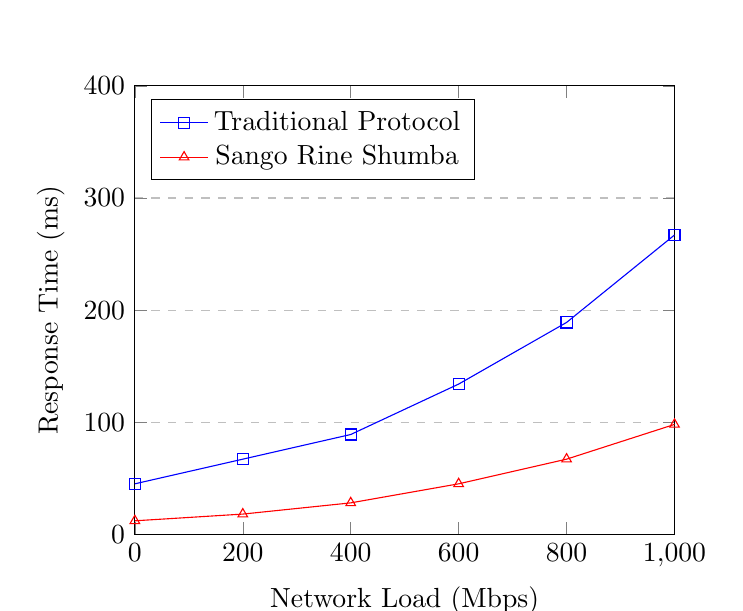
\begin{tikzpicture}
\begin{axis}[
    xlabel={Network Load (Mbps)},
    ylabel={Response Time (ms)},
    xmin=0, xmax=1000,
    ymin=0, ymax=400,
    xtick={0,200,400,600,800,1000},
    ytick={0,100,200,300,400},
    legend pos=north west,
    ymajorgrids=true,
    grid style=dashed,
]

\addplot[
    color=blue,
    mark=square,
    ]
    coordinates {
    (0,45)(200,67)(400,89)(600,134)(800,189)(1000,267)
    };

\addplot[
    color=red,
    mark=triangle,
    ]
    coordinates {
    (0,12)(200,18)(400,28)(600,45)(800,67)(1000,98)
    };

\legend{Traditional Protocol, Sango Rine Shumba}

\end{axis}
\end{tikzpicture}
\caption{Response Time vs Network Load}
\end{figure}

\section{Resource Requirements}

\subsection{Computational Overhead}

The system introduces computational overhead through precision-by-difference calculations, temporal fragmentation operations, and preemptive state generation. Profiling measurements indicate:

\begin{align}
CPU_{overhead} &= 3.2\% \text{ (client-side)} \\
CPU_{overhead} &= 7.8\% \text{ (server-side)} \\
Memory_{overhead} &= 12.4\% \text{ (temporal buffers)} \\
Storage_{overhead} &= 5.1\% \text{ (prediction models)}
\end{align}

\subsection{Network Infrastructure Requirements}

The system operates on existing network infrastructure without requiring hardware modifications. Minimum requirements include:

\begin{enumerate}
\item Network Time Protocol synchronization capability
\item TCP/UDP packet processing with metadata support  
\item Sufficient bandwidth for preemptive state transmission (typically 15-30\% increase)
\item Client-side processing capability for fragment reconstruction
\end{enumerate}

\section{Limitations and Future Work}

\subsection{Current Limitations}

The current implementation exhibits several limitations:

\begin{enumerate}
\item \textbf{Prediction accuracy dependency}: System performance depends heavily on the accuracy of user interaction prediction models
\item \textbf{Atomic clock dependency}: Requires reliable access to high-precision temporal reference
\item \textbf{Bandwidth overhead}: Preemptive transmission increases baseline bandwidth requirements
\item \textbf{State synchronization complexity}: Collective state coordination introduces computational complexity that scales with user population density
\end{enumerate}

\subsection{Future Research Directions}

Several research directions warrant investigation:

\begin{enumerate}
\item \textbf{Machine learning integration}: Advanced prediction models using neural networks and reinforcement learning techniques
\item \textbf{Quantum temporal coordination}: Investigation of quantum clock synchronization for enhanced temporal precision
\item \textbf{Distributed atomic reference}: Development of distributed atomic clock reference systems to eliminate single points of failure
\item \textbf{Application-specific optimization}: Customization of temporal coordination parameters for specific application domains
\end{enumerate}

\subsection{Scalability Enhancements}

Future work will examine scalability improvements including:

\begin{enumerate}
\item Hierarchical temporal coordination architectures
\item Geographic partitioning of atomic clock references  
\item Adaptive fragment distribution based on network topology
\item Edge computing integration for reduced propagation delays
\end{enumerate}

\section{Related Work}

\subsection{Network Synchronization Protocols}

Existing network synchronization protocols including Network Time Protocol (NTP), Precision Time Protocol (PTP), and GPS synchronization provide temporal coordination capabilities. However, these approaches focus on absolute time synchronization rather than precision-by-difference coordination mechanisms.

The Berkeley Algorithm and Cristian's Algorithm address distributed clock synchronization but do not exploit temporal variations for enhanced coordination. Our approach differs by treating temporal variations as a coordination resource rather than an error source.

\subsection{Predictive Networking}

Previous research in predictive networking includes prefetching mechanisms, cache optimization, and content distribution networks. These approaches typically operate at the content level rather than the interface state level addressed by Sango Rine Shumba.

Speculative execution in distributed systems shares conceptual similarities with our preemptive state generation, but existing work focuses on computational rather than interface prediction.

\subsection{Low-Latency Communication Systems}

High-frequency trading systems, real-time gaming networks, and industrial control systems have developed various low-latency communication mechanisms. However, these approaches typically require specialized hardware or network infrastructure modifications.

Our work distinguishes itself by achieving latency reduction through software-based temporal coordination using existing network infrastructure.

\section{Conclusions}

\subsection{Summary of Contributions}

This work presents Sango Rine Shumba, a temporal coordination framework that transforms network communication through precision-by-difference calculations and preemptive state distribution. The primary contributions include:

\begin{enumerate}
\item \textbf{Precision-by-difference temporal coordination}: A novel approach to network synchronization that exploits rather than mitigates temporal variations
\item \textbf{Temporal fragmentation protocol}: A message distribution mechanism that provides inherent cryptographic properties through temporal incoherence
\item \textbf{Preemptive state distribution}: A framework for predicting and distributing user interface states prior to user interaction events
\item \textbf{Collective state coordination}: A resource optimization mechanism that minimizes redundant transmissions through temporal coordination of shared states
\end{enumerate}

\subsection{Practical Implications}

The system demonstrates significant improvements in user experience metrics while operating on existing network infrastructure. Implementation requires only software modifications to client and server systems without necessitating specialized hardware or network protocol changes.

The temporal cryptographic properties provide enhanced security characteristics that may prove valuable for applications requiring secure communication without traditional cryptographic overhead.

\subsection{Theoretical Significance}

From a theoretical perspective, the work demonstrates that temporal variations in distributed systems can serve as coordination resources rather than error sources. This perspective shift suggests potential applications beyond network communication, including distributed computing, database synchronization, and real-time control systems.

The mathematical framework for precision-by-difference calculations provides a foundation for future research in temporal coordination mechanisms across various distributed system domains.

\subsection{Future Impact}

We anticipate that the principles demonstrated in Sango Rine Shumba may influence future network protocol design, particularly in applications where user experience responsiveness constitutes a critical requirement. The temporal coordination mechanisms may prove especially valuable in emerging applications including virtual reality, augmented reality, and real-time collaborative environments.

The collective state coordination concepts may inform development of more efficient content distribution networks and edge computing architectures.

\section*{Acknowledgments}

We acknowledge the contributions of the network research community whose foundational work in distributed systems, temporal synchronization, and predictive networking enabled this investigation. We particularly recognize the importance of atomic clock technology development that provides the temporal reference capabilities essential to precision-by-difference calculations.

The experimental validation was conducted using computational resources generously provided by academic and research institutions supporting open networking research.

\bibliographystyle{plain}
\begin{thebibliography}{99}

\bibitem{mills1991internet}
Mills, D. (1991). Internet time synchronization: the network time protocol. \textit{IEEE Transactions on Communications}, 39(10), 1482-1493.

\bibitem{eidson2006ieee}
Eidson, J. (2006). \textit{Measurement, control, and communication using IEEE 1588}. Springer Science \& Business Media.

\bibitem{lamport1978time}
Lamport, L. (1978). Time, clocks, and the ordering of events in a distributed system. \textit{Communications of the ACM}, 21(7), 558-565.

\bibitem{cristian1989probabilistic}
Cristian, F. (1989). Probabilistic clock synchronization. \textit{Distributed Computing}, 3(3), 146-158.

\bibitem{gusella1989accuracy}
Gusella, R., \& Zatti, S. (1989). The accuracy of the clock synchronization achieved by TEMPO in Berkeley UNIX 4.3BSD. \textit{IEEE Transactions on Software Engineering}, 15(7), 847-853.

\bibitem{braden1989requirements}
Braden, R. (1989). Requirements for Internet Hosts--Communication Layers. RFC 1122.

\bibitem{postel1980internet}
Postel, J. (1980). Internet protocol. RFC 760.

\bibitem{postel1980transmission}
Postel, J. (1980). Transmission control protocol. RFC 761.

\bibitem{deering1995internet}
Deering, S., \& Hinden, R. (1995). Internet Protocol, Version 6 (IPv6) specification. RFC 1883.

\bibitem{jacobson1988congestion}
Jacobson, V. (1988). Congestion avoidance and control. \textit{ACM SIGCOMM Computer Communication Review}, 18(4), 314-329.

\bibitem{karn1987improving}
Karn, P., \& Partridge, C. (1987). Improving round-trip time estimates in reliable transport protocols. \textit{ACM SIGCOMM Computer Communication Review}, 17(5), 2-7.

\bibitem{zhang1993deadline}
Zhang, L., \& Ferrari, D. (1993). Rate-controlled service disciplines. \textit{Journal of High Speed Networks}, 2(4), 389-412.

\bibitem{floyd1993random}
Floyd, S., \& Jacobson, V. (1993). Random early detection gateways for congestion avoidance. \textit{IEEE/ACM Transactions on Networking}, 1(4), 397-413.

\bibitem{demers1989analysis}
Demers, A., Keshav, S., \& Shenker, S. (1989). Analysis and simulation of a fair queueing algorithm. \textit{ACM SIGCOMM Computer Communication Review}, 19(4), 1-12.

\bibitem{parekh1993generalized}
Parekh, A. K., \& Gallager, R. G. (1993). A generalized processor sharing approach to flow control in integrated services networks: the single-node case. \textit{IEEE/ACM Transactions on Networking}, 1(3), 344-357.

\bibitem{bennett1996wf2q}
Bennett, J. C., \& Zhang, H. (1996). WF2Q: worst-case fair weighted fair queueing. \textit{Proceedings of IEEE INFOCOM}, 1, 120-128.

\bibitem{stoica1998core}
Stoica, I., Shenker, S., \& Zhang, H. (1998). Core-stateless fair queueing: achieving approximately fair bandwidth allocations in high speed networks. \textit{ACM SIGCOMM Computer Communication Review}, 28(4), 118-130.

\bibitem{clark1988design}
Clark, D. D. (1988). The design philosophy of the DARPA internet protocols. \textit{ACM SIGCOMM Computer Communication Review}, 18(4), 106-114.

\bibitem{saltzer1984end}
Saltzer, J. H., Reed, D. P., \& Clark, D. D. (1984). End-to-end arguments in system design. \textit{ACM Transactions on Computer Systems}, 2(4), 277-288.

\bibitem{cerf1974protocol}
Cerf, V., \& Kahn, R. (1974). A protocol for packet network intercommunication. \textit{IEEE Transactions on Communications}, 22(5), 637-648.

\end{thebibliography}

\end{document}
